% =============================================================================
\section{Results}
% =============================================================================

\begin{frame}{Project goal}
  \small
  \textbf{Research question:} Can NLP map an unstructured chief complaint to the correct acuity level and colour-coded clinical pathway?

  \vspace{0.15cm}
  \begin{block}{Formal objective}
    \[
      \text{Input } X \;\to\; \hat{c} \in \{1,\ldots,5\} \;\to\; C = f_{\mathrm{SATS}}(\hat{c})
    \]
  \end{block}

  \textbf{What it does:} converts patient text into an acuity level, then into a SATS colour for routing.

  \vartable{
    $X$ & Chief complaint text & Raw patient input (max 128 tokens) \\
    $\hat{c}$ & Predicted acuity level & Model output before colour mapping \\
    $C$ & SATS colour & Red / Orange / Yellow / Green pathway \\
    $f_{\mathrm{SATS}}$ & Level-to-colour map & Fixed rule: $1\!\to\!$Red, $2\!\to\!$Orange, $3\!\to\!$Yellow, $4,5\!\to\!$Green \\
  }
\end{frame}

\begin{frame}{Was the goal achieved?}
  \small
  \begin{block}{Answer: Yes --- on 8{,}000-sample holdout}
    \textbf{99.92\%} of complaints were routed to the correct SATS colour (baseline BioBERT).
  \end{block}

  \vspace{0.1cm}
  \begin{itemize}
    \item 7,994 of 8,000 complaints: predicted colour matches nurse label
    \item 6 errors on Level 1 (Red) --- the most critical safety class
    \item Holdout = 10\% stratified split the model did not train on
  \end{itemize}

  \plain{Because $f_{\mathrm{SATS}}$ is a fixed mapping, getting the acuity level right means getting the colour pathway right. Next slide defines the accuracy formula and every symbol.}
\end{frame}

\begin{frame}{Variables: colour-routing accuracy}
  \small
  \textbf{What it computes:} the fraction of patients routed to the correct colour.

  \vspace{0.1cm}
  \[
    P\!\left(f_{\mathrm{SATS}}(\hat{c}) = f_{\mathrm{SATS}}(c_{\mathrm{nurse}})\right) = 0.9992
  \]
  \[
    \mathrm{Accuracy} = \frac{1}{n}\sum_{i=1}^{n} \mathbb{1}\!\left[\hat{c}_i = c_i\right] = 0.9992
  \]

  \vartable{
    $\hat{c}_i$ & Model's predicted level for patient $i$ & BioBERT output before colour map \\
    $c_i$ & Nurse's true acuity label & Ground truth from training data \\
    $c_{\mathrm{nurse}}$ & Same as $c_i$ (one patient) & Reference label to compare against \\
    $n$ & Number of test complaints & $n = 8{,}000$ on holdout \\
    $\mathbb{1}[\cdot]$ & Indicator function & $=1$ if prediction correct, $=0$ if wrong \\
    $f_{\mathrm{SATS}}$ & Level $\to$ colour function & Turns level into routing colour \\
  }

  \textbf{Result:} $\frac{7994}{8000} = 0.9992$.
\end{frame}

\begin{frame}{How we measure success}
  \footnotesize
  We tested on \textbf{8,000 complaints} the model had not seen during training (10\% stratified holdout).

  \vspace{0.08cm}
  \begin{columns}[T]
    \column{0.46\textwidth}
    \begin{tabular}{@{}p{1.9cm} p{3.4cm}@{}}
      \toprule
      \textbf{Metric} & \textbf{Simple formula} \\
      \midrule
      Accuracy &
      $\dfrac{\text{correct}}{\text{total}} = \dfrac{7994}{8000}$ \\[3pt]
      Precision &
      $\dfrac{TP}{TP + FP}$ \\[3pt]
      Recall &
      $\dfrac{TP}{TP + FN}$ \\[3pt]
      F1 &
      $2 \cdot \dfrac{\text{Prec} \cdot \text{Rec}}{\text{Prec} + \text{Rec}}$ \\[3pt]
      Macro-F1 &
      average F1 across all 5 levels \\
      \bottomrule
    \end{tabular}

    \column{0.50\textwidth}
    \textbf{What each one measures:}
    \begin{itemize}\setlength{\itemsep}{2pt}
      \item \textbf{Accuracy} --- overall correct routing rate
      \item \textbf{Precision} --- when we say ``Red'', how often correct?
      \item \textbf{Recall} --- of all real Reds, how many caught?
      \item \textbf{F1} --- balance of precision and recall
      \item \textbf{Macro-F1} --- each level weighted equally
    \end{itemize}
  \end{columns}

  \examplebox{
    Next slide defines $TP$, $FP$, $FN$ and how they enter precision and recall.
  }
\end{frame}

\begin{frame}{Variables: TP, FP, FN}
  \footnotesize
  \textbf{What they count} (for one acuity class, e.g.\ Level 1 Red):

  \vartable{
    $TP$ & True positives & Correctly predicted as this class \\
    $FP$ & False positives & Wrongly predicted as this class \\
    $FN$ & False negatives & This class missed by the model \\
  }

  \vspace{0.15cm}
  \textbf{Example (L1 Red):} 322 true Reds; model correctly flags 316 ($TP$) and misses 6 ($FN$); no false Reds ($FP=0$).
\end{frame}

\begin{frame}{Variables: Precision, Recall, Macro-F1}
  \footnotesize
  \textbf{What the formulas compute:} per-class quality and an average across all five levels.

  \vartable{
    Prec & $TP/(TP+FP)$ & When we predict this class, how often right? \\
    Rec & $TP/(TP+FN)$ & Of all true cases, how many did we catch? \\
    $F1$ & $2\cdot\frac{\text{Prec}\cdot\text{Rec}}{\text{Prec}+\text{Rec}}$ & Single score balancing both \\
    Macro-F1 & $\frac{1}{5}\sum_{c=1}^{5} F1_c$ & Each level weighted equally \\
  }

  \vspace{0.08cm}
  \[
    \mathrm{Precision}_c = \frac{TP_c}{TP_c + FP_c}, \qquad
    \mathrm{Recall}_c = \frac{TP_c}{TP_c + FN_c}
  \]

  \plain{Macro-F1 averages F1 across all 5 levels so minority classes (Red) count as much as majority (Yellow).}
\end{frame}

\begin{frame}{Model performance: baseline vs SMOTE}
  \small
  \textbf{Default inference model:} baseline BioBERT.

  \vspace{0.1cm}
  \begin{table}
    \centering
    \footnotesize
    \begin{tabular}{@{}lrr@{}}
      \toprule
      \textbf{Metric} & \textbf{Baseline} & \textbf{SMOTE} \\
      \midrule
      Accuracy & 99.92\% & 99.85\% \\
      Macro-F1 & 99.77\% & 99.54\% \\
      Recall L1 (Red) & 98.14\% & 100.00\% \\
      Mean confidence $\bar{c}$ & 0.9997 & 0.9992 \\
      Predictions with $\hat{y}_{\hat{c}} = 1.0$ & 79.05\% & 82.99\% \\
      Latency p50 (ms/sample) & 100.3 & 95.5 \\
      \bottomrule
    \end{tabular}
  \end{table}

  \vartable{
    $\bar{c}$ & Mean softmax confidence & Average of top-class probabilities \\
    $\hat{y}_{\hat{c}}$ & Confidence of predicted class & How sure the model is about its pick \\
    SMOTE & Oversampled training variant & Alternative model for minority-class recall \\
  }
\end{frame}

\begin{frame}{Worked example: L1 Red recall}
  \small
  \textbf{What it computes:} of all true Red patients, what fraction did we correctly route to Red?

  \vspace{0.1cm}
  \[
    \mathrm{Rec}_{\mathrm{L1}} = \frac{TP_{\mathrm{L1}}}{TP_{\mathrm{L1}} + FN_{\mathrm{L1}}}
    = \frac{316}{322} = 0.9814
  \]

  \vartable{
    $TP_{\mathrm{L1}}$ & True Red cases correctly predicted Red & 316 patients \\
    $FN_{\mathrm{L1}}$ & True Red cases missed (wrong colour) & 6 patients \\
    $322$ & Total true Red in holdout & Support count for Level 1 \\
    $\mathrm{Rec}_{\mathrm{L1}}$ & L1 recall & Safety metric: missed emergencies \\
  }

  \plain{Six Red patients were assigned a less urgent colour --- the main clinical risk on this holdout.}
\end{frame}

\begin{frame}{Per-class results and confusion matrix}
  \footnotesize
  \begin{columns}[T]
    \column{0.46\textwidth}
    \textbf{Baseline per-class}
    \vspace{0.06cm}
    \begin{tabular}{@{}lrrrr@{}}
      \toprule
      \textbf{Class} & \textbf{Prec} & \textbf{Rec} & \textbf{F1} & $n$ \\
      \midrule
      L1 Red & 1.00 & 0.98 & 0.99 & 322 \\
      L2 Orange & 1.00 & 1.00 & 1.00 & 1344 \\
      L3 Yellow & 1.00 & 1.00 & 1.00 & 2892 \\
      L4 Green & 1.00 & 1.00 & 1.00 & 2302 \\
      L5 Green & 1.00 & 1.00 & 1.00 & 1140 \\
      \bottomrule
    \end{tabular}

    \vspace{0.1cm}
    \textbf{Confusion matrix:} $\sum_i C_{ii} = 7{,}994$ correct; 6 off-diagonal errors.

    \column{0.50\textwidth}
    \begin{center}
      \IfFileExists{../eval_outputs/baseline_confusion.png}{%
        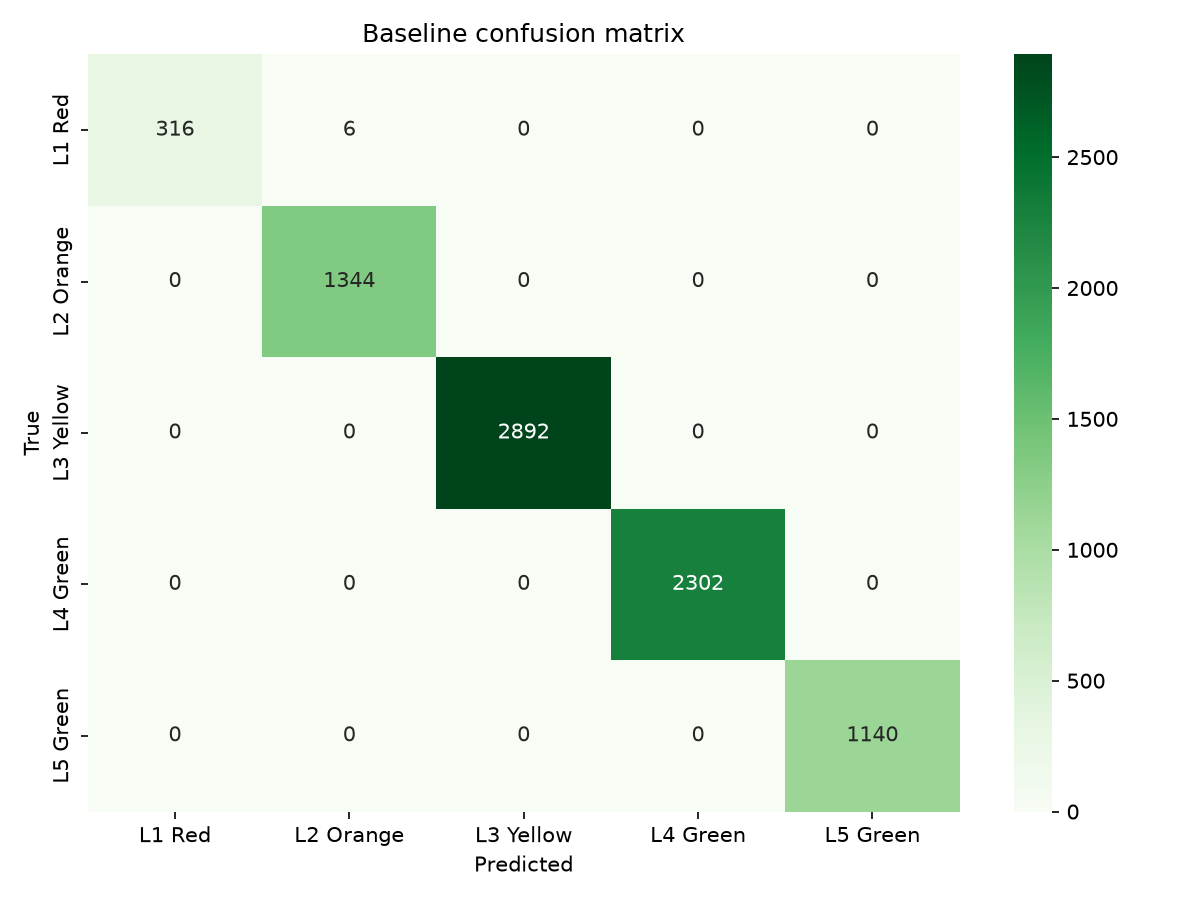
\includegraphics[width=\textwidth]{../eval_outputs/baseline_confusion.png}%
      }{%
        \textit{Confusion matrix not found}%
      }
    \end{center}
  \end{columns}
\end{frame}

\begin{frame}{Variables: confusion matrix}
  \footnotesize
  \textbf{What it shows:} how many patients with true level $i$ were predicted as level $j$.

  \vartable{
    $C_{ij}$ & Count: true level $i$, predicted $j$ & Cell in confusion matrix \\
    $C_{ii}$ & Diagonal entries & Correct routing (same level) \\
    $i,j$ & Class indices $1,\ldots,5$ & Rows = truth, columns = prediction \\
    $n$ & Row sum $\sum_j C_{ij}$ & Number of true cases per class \\
  }

  \textbf{Result:} $\sum_i C_{ii} = 7{,}994$ correct; all 6 errors involve true Level 1 (Red).
\end{frame}

\begin{frame}{Variables: model confidence}
  \small
  \textbf{What it computes:} how strongly the softmax favours the predicted class.

  \vspace{0.1cm}
  \[
    \hat{y}_{\hat{c}} = \max_{c \in \{1,\ldots,5\}} \hat{y}_c, \qquad
    \bar{c} = \frac{1}{n}\sum_{i=1}^{n} \hat{y}_{\hat{c}_i}
  \]

  \vartable{
    $\hat{y}_c$ & Softmax probability for level $c$ & Model belief for each class; $\sum_c \hat{y}_c = 1$ \\
    $\hat{c}$ & $\arg\max_c \hat{y}_c$ & Predicted acuity level (highest probability) \\
    $\hat{y}_{\hat{c}}$ & Probability of the predicted class & Confidence score shown in the app \\
    $\bar{c}$ & Mean confidence over $n$ samples & Average certainty on holdout ($=0.9997$) \\
    $n$ & Holdout size & $n = 8{,}000$ complaints \\
  }

  \textbf{Result:} 79.05\% of predictions have $\hat{y}_{\hat{c}} = 1.0$ exactly.
\end{frame}

\begin{frame}{Calibration results}
  \small
  \textbf{What calibration means:} when the model says 90\% confident, it should be right $\sim$90\% of the time. Our model is \textbf{overconfident}.

  \begin{columns}[T]
    \column{0.44\textwidth}
    \begin{center}
      \IfFileExists{../eval_outputs/baseline_calibration.png}{%
        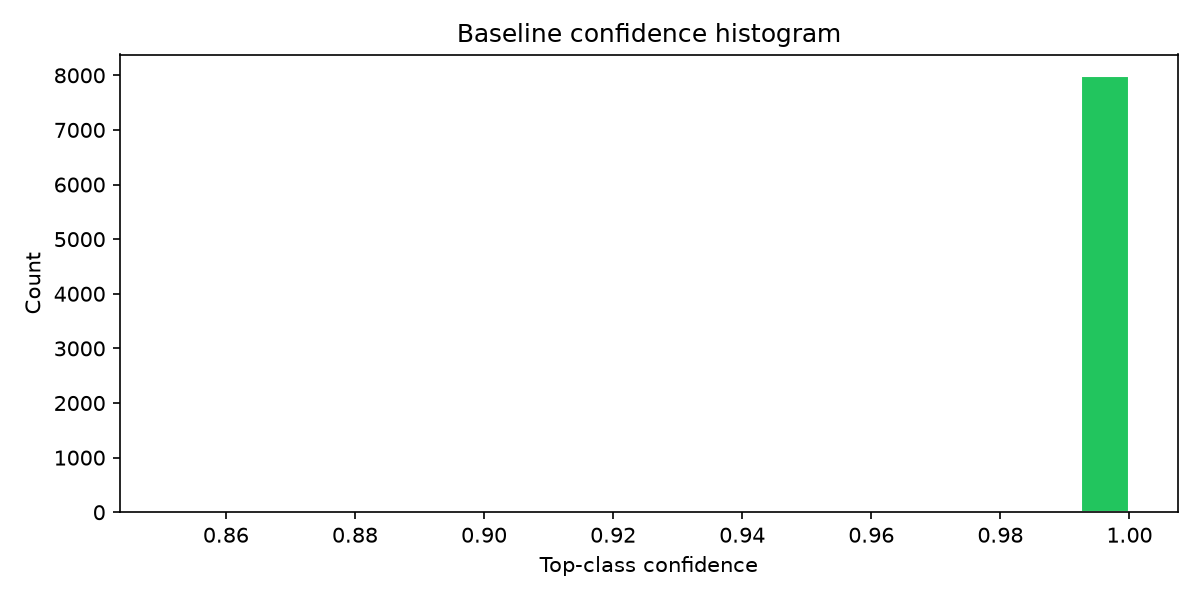
\includegraphics[width=\textwidth]{../eval_outputs/baseline_calibration.png}%
      }{%
        \textit{Calibration plot not found}%
      }
    \end{center}

    \column{0.52\textwidth}
    \begin{itemize}
      \item $\bar{c} = 0.9997$ --- very high mean confidence
      \item $P(\hat{y}_{\hat{c}} = 1.0) = 0.7905$ --- 79\% at maximum
      \item $P(\hat{y}_{\hat{c}} < \tau) = 0$ where $\tau = 0.85$
    \end{itemize}
  \end{columns}
\end{frame}

\begin{frame}{Variables: calibration threshold}
  \footnotesize
  \textbf{What these symbols mean for deployment safety:}

  \vartable{
    $\tau$ & Confidence threshold & Below $\tau$, flag for Bayesian / manual review \\
    $P(\cdot)$ & Probability over holdout & Fraction of predictions meeting a condition \\
    Calibration & Confidence vs correctness & Miscalibration = trusting softmax too much \\
  }

  \plain{Cross-entropy training rewards confident correct answers, so probabilities cluster near 1.0. TEWS vitals remain essential for safe triage.}
\end{frame}

\begin{frame}{Goal vs evidence}
  \small
  \begin{columns}[T]
    \column{0.48\textwidth}
    \begin{block}{Goal}
      \begin{itemize}
        \item Predict acuity level from text
        \item Route patient to correct SATS colour
        \item Support colour-coded clinical pathways
      \end{itemize}
    \end{block}

    \column{0.48\textwidth}
    \begin{block}{Evidence (baseline)}
      \begin{itemize}
        \item Accuracy: \textbf{99.92\%}
        \item Macro-F1: \textbf{99.77\%}
        \item L1 (Red) recall: \textbf{98.14\%}
        \item Colour routing: \textbf{7,994 / 8,000} correct
      \end{itemize}
    \end{block}
  \end{columns}

  \vspace{0.15cm}
  \textbf{Limitations:}
  \begin{itemize}
    \item Holdout is in-distribution --- live KATH data may differ
    \item 79\% of predictions overconfident ($\hat{y}_{\hat{c}} = 1.0$)
    \item Text-only --- vitals (TEWS) needed for full clinical safety
  \end{itemize}
\end{frame}

\begin{frame}{Conclusion}
  \small
  \textbf{Pipeline recap:}
  complaint $\to$ tokenize $\to$ embed $\to$ BioBERT $\to$ acuity level $\to$ SATS colour $\to$ clinical pathway.

  \vspace{0.15cm}
  \begin{enumerate}
    \item The goal --- \textbf{acuity prediction and colour-coded routing} --- was achieved at 99.92\% on holdout
    \item Baseline BioBERT is the default model (99.77\% macro-F1)
    \item The open mathematical problem is \textbf{calibration}: softmax overconfidence means TEWS vitals and Bayesian fusion remain essential safety layers
  \end{enumerate}

  \vspace{0.3cm}
  \centering
  \Large\textbf{Questions?}
\end{frame}
